

\chapter{Data Set}
\section{Labelled Pupils in the Wild (LPW)}
\subsection{Description}

The data set "Labelled Pupils in the Wild" \cite{zhang_max-planck-institut_2016}, or short LPW, was created by the Max Plank Institut and contains 66 high-quality, high-speed eye region videos for developing and evaluating pupil detection algorithms. All videos are labeled with the center of the pupil. Twenty-two participants with five different ethnicities and eye colors volunteered to record their eye movements.  

The data set's goal was to record eye movement under natural conditions. With strong reflections, wearing glasses and wearing makeup, the data set becomes a difficult challenge for pupil detection algorithms and a good evaluation of algorithms is possible.


\begin{figure}[ht]
    \centering
    \begin{subfigure}{.30\textwidth}
      \centering
      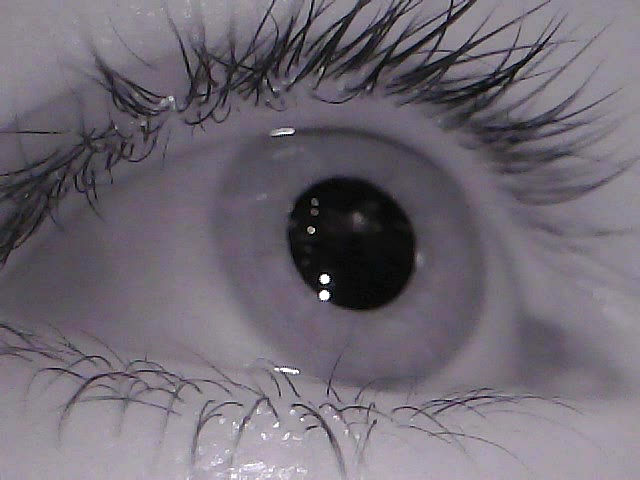
\includegraphics[width=.9\linewidth]{plots/eye_dataset/eye1.png}

      \label{fig:ds1}
    \end{subfigure}%
    \begin{subfigure}{.30\textwidth}
      \centering
      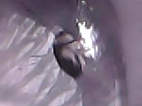
\includegraphics[width=.9\linewidth]{plots/eye_dataset/eye2.png}

      \label{fig:ds2}
    \end{subfigure}%
    \begin{subfigure}{.30\textwidth}
      \centering
      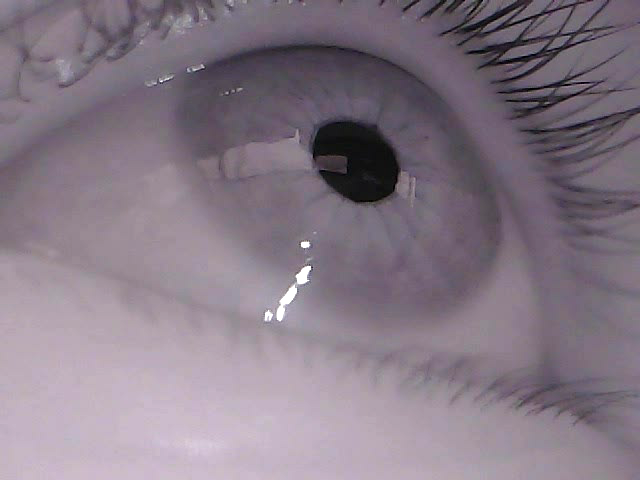
\includegraphics[width=.9\linewidth]{plots/eye_dataset/eye3.png}

      \label{fig:ds3}
    \end{subfigure}
    \caption{Three example frames from the LPW data set.}
    \label{fig:example_frame}
    \end{figure}

    \subsection{Procedure}
    The participants were asked to look at a red ball as it moved around. The recording location was randomly picked around several buildings. Each location was chosen once, creating a diverse range of real-life situations. 

    For the recording, a high-speed Pupil Pro head-mounted eye tracker took 95 frames per second with a resolution of 640x480 pixels. With this frame rate, even fast eye movements last through several frames, making it more robust to detect the pupil. 


    \begin{table}[h]
      \centering 
      \begin{minipage}{0.7\textwidth}
        \centering
        \begin{tabular}{|c|c|}
          \hline
          Location & Number of Videos \\
          \hline
          Outside & 34.3\% \\
          Inside & 65.7\% \\
          \hline
        \end{tabular}
        \caption{Location of recordings}
        \label{tab:location}
      \end{minipage}\hfill
      \begin{minipage}{0.7\textwidth}
        \centering
        \begin{tabular}{|c|c|}
          \hline
          Light source & Percentage of recordings \\
          \hline
          Natural light & 84.7\% \\
          Artificial light & 33.6\% \\
          \hline
        \end{tabular}
        \caption{Light Source of recordings}
        \label{tab:light_source}
      \end{minipage}
    \end{table}

    \subsection{Ground truth annotation}
    \label{subsec:ground_truth}
    In many cases, the pupil area has a clear distinctive boundary and the center can be annotated easily. If the boundary was incomplete, one or two points inside the pupil were manually selected and used as seed points. From these points, the area with the same intensity value is extracted and used for annotation.  However, this method was not possible in challenging scenarios because of the strong noise over the pupil. In this case, additional information was retrieved from the participants following a red ball with their eyes. This data was then used as calibration data to cross-reference the center of the pupil according to the position of the red ball and the eye movement. 
    
    The complete data set has ground truth annotations of the pupil's center for every frame.
    Given the ground truth annotation, it is possible to evaluate algorithms and compare them to each other.
    \subsection{Folder structure}
    The folder structure of the data set is straightforward. The data set is divided into 22 folders, one for each participant. Each participant folder contains three recordings in different locations with different light sources with their corresponding text file.
    The text file contains the ground truth annotation of the pupil center in x and y coordinates for each frame and more information about the participant. 
    
    The labels.ods file contains information about the location, light source, vision aid used, prescription, nationality, eye color and gender. The README.txt file contains the information about the data set and the folder structure.
    \newpage
    \section{Eye characteristics}
    \subsection{Anatomy of the eye}
    The eye is surrounded by the \textbf{eye lid}. Its purpose is to shield the eye from debris and lubricate the eye by spreading tears fluid over its surface with each blink. Four different parts of the eye matter for pupil detection. As seen in figure \ref{fig:eye_anatomy}.
    \begin{figure}[h]
      \centering
      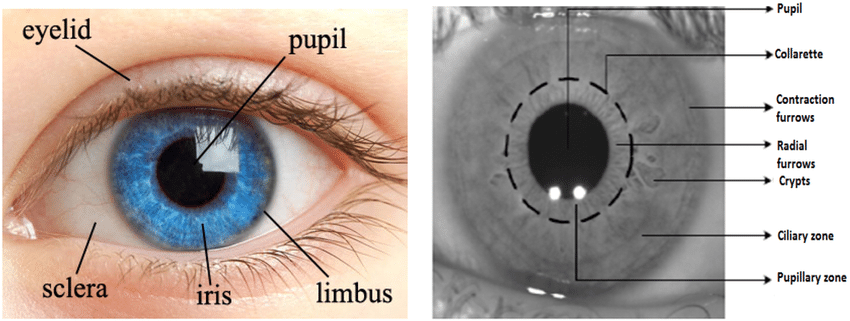
\includegraphics[width=0.98\textwidth]{plots/eye_dataset/Various-characteristics-of-an-eye-and-its-iris-texture-7.png}
      \caption{Overview of the different parts of the eye. \cite{noauthor_various_2009}}
      \label{fig:eye_anatomy}
    \end{figure}
    
    The white part of the eye is the \textbf{sclera} and is separated from the \textbf{iris} by the \textbf{limbus}. The table \ref{tab:eye_char} shows the size difference between the iris and the pupil \cite{drahansky_recognition_2018}
    \begin{table}[h]
      \centering 
      \begin{minipage}{0.7\textwidth}
        \centering
        \begin{tabular}{|c|c|c|}
          \hline
          Name & Radius & Additional Information \\
          \hline
          Iris & 12 mm & in average\\
          Pupil & 2-9 mm & varies with light intensity\\
          \hline
        \end{tabular}
        \caption{Oversight iris and pupil radius}
        \label{tab:eye_char}
      \end{minipage}\hfill
    \end{table}
 

    The iris regulates the radius size of the \textbf{pupil}, thereby regulating how much light comes through the pupil. The pupil is in the center of the iris and is the black part of the eye. The Darker the environment is, the larger the pupil radius. The iris is colored and can be blue, green/hazel, brown, gray, amber and black. There are also other colors that are connected with health issues or genetic defects and play no role in this thesis. 

    The critical fact for pupil detection is that the iris, pupil and sclera have different brightness intensity values. The pupil is the darkest area in the eye, the sclera is the brightest and the iris is something in between. Depending on the color of the iris, the brightness value can vary. Those characteristics are often used in pupil detection algorithms and will be discussed in the next chapter.

    There can also be reflections of the environment that can be seen in the eye. This reflection is called \textbf{corneal reflection} and can temper with pupil detection algorithms accuracy and therefore is a challenge for pupil detection algorithms.


    \subsection{Image characteristics}
    \subsubsection{Histogram}
    When inspecting the histogram of a randomly chosen frame from the LPW data set, the histogram has peaks in different intensities. In figure \ref{fig:hist1}, the peak between 0 and 50 corresponds to the pupil. This becomes clear, when comparing the histograms of the whole image with the region of interest (ROI), the lowest peak stays unchanged. The intensity of the iris is therefore between 90 and 150.

    \begin{figure}[ht]
      \centering
      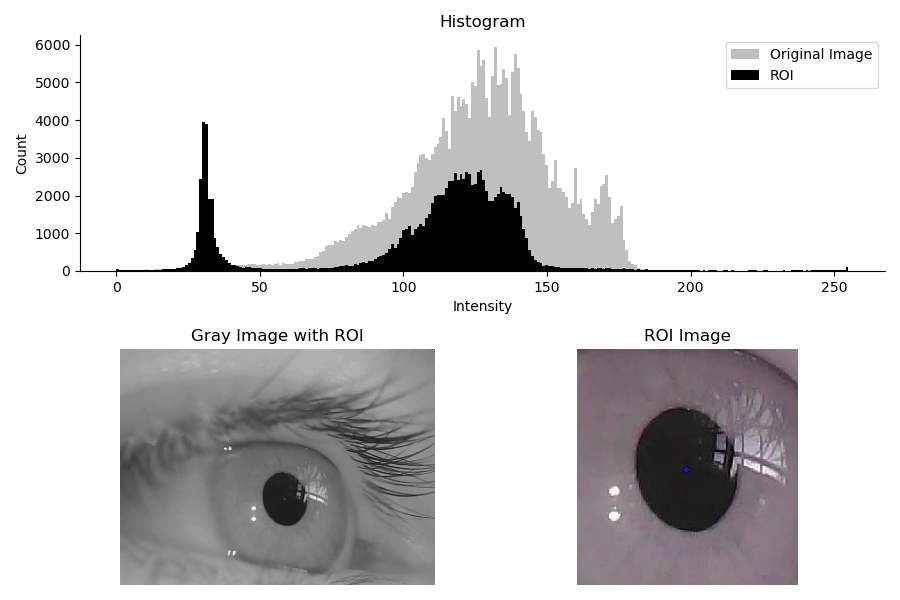
\includegraphics[width=0.9\textwidth]{plots/histogram_with_roi.png}
      \caption{Comparing the histogram of the whole image and the region of interest.}
      \label{fig:hist1}
    \end{figure}

    The sclera is the brightest part of the eye, but in this frame, the skin intensity will be around the same magnitude as the sclera intensity. 

    If there is more reflection on the pupil, the histogram will also change shape. The peak created by the pupil will shrink and flatten out. The mean of the histogram will increase as dark points are substituted by brighter points. The presence of corneal reflection ultimately makes it hard to use a fixed threshold for segmentation. Using Histogram equalization increases the contrast of the image but stretches the peak into a wider intensity range. 

    Also interesting to inspect is a single pixel row of the image with their intensity values. Here it can be observed that the pupil creates a valley in the intensity values and the reflection on the pupil generates a peak right after or in the valley. The row intensity is shown in figure \ref{fig:row_intens}.
    \begin{figure}[ht]
      \centering
      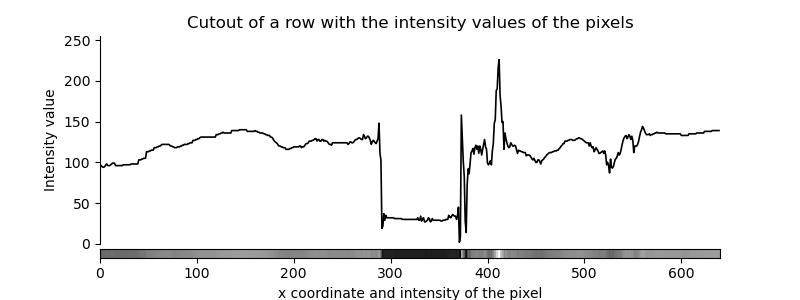
\includegraphics[width=0.9\textwidth]{plots/row_intensity_valles.png}
      \caption{Plot of the intensity values of one pixel row.}
      \label{fig:row_intens}
    \end{figure}

    The x coordinate of figure \ref{fig:row_intens} represents the pixel at this coordination and the y coordinate represents the intensity value of the pixel. 

    The conclusion is, that the histogram is a solid tool to gain information about the pupil, but can vary a lot depending on the environment. Therefore adaptive algorithms have to be used. 
    
    \subsubsection{Noise}
      In the data set there are different kinds of noise. The most obvious one is the \textbf{corneal reflection}. The environment reflects on the eye and is seen as a bright spot on the pupil and destroys information of the pupil. Also \textbf{eyelashes} can be problematic as they are very dark and are often between the camera and the pupil. 

      Another Noise term can be that the eye is not constantly open. The \textbf{eyelid} can cover parts of the pupil or even the whole pupil. Glasses or lenses can add noise to the image as well as when the camera's focus is not on the pupil.